\documentclass[11pt]{article}
\usepackage[margin=1in]{geometry}
\usepackage{amsmath,amssymb,amsthm,booktabs,graphicx}
\usepackage[colorlinks=true,linkcolor=blue,urlcolor=blue,citecolor=blue]{hyperref}
\newtheorem{theorem}{Theorem}[section]
\newtheorem{proposition}[theorem]{Proposition}
\newtheorem{corollary}[theorem]{Corollary}
\newtheorem{remark}[theorem]{Remark}
\newcommand{\R}{\mathbb R}
\newcommand{\E}{\mathbb E}
\newcommand{\ip}[2]{\langle #1,#2\rangle}
\newcommand{\F}[1]{\lVert #1\rVert_{\mathrm F}}
\newcommand{\nuc}[1]{\lVert #1\rVert_*}
\newcommand{\op}[1]{\lVert #1\rVert_{\mathrm{op}}}
\newcommand{\ent}[1]{\lVert #1\rVert_{1,\mathrm{entry}}}
\newcommand{\sgn}{\operatorname{sign}}
\newcommand{\rank}{\operatorname{rank}}
\newcommand{\pos}[1]{[#1]_+}
\title{Fanions at every rank:\\finite budgets, hybrid crossovers, and Nesterov tracking}
\author{Second research attempt for the Neon repository}
\date{21 October 2026}
\begin{document}
\maketitle

\begin{abstract}
We extend the comparison to every rank $k$ in the plain, F-, and S-Fanion
families. A single convergence theorem retains their different support
functions, gradient spectra, entry density, cumulative learning rates, and
oracle errors. Its momentum corollary uses the repository's actual Nesterov
convention. We strengthen the quadratic lower bounds by retaining the whole
initial singular spectrum and by separating a hybrid's rank-limited and dense
updates. An exactly solvable spectral flow explains both $1/k$ progress and
its saturation; hybrid examples identify different crossover ranks.
The saved quadratic traces provide unusually close evidence for the low-rank
time scale: Fanion-2 and Fanion-10 nearly coincide with Neon after rescaling
time by $k$. A source audit also finds a different learning-rate schedule for
F-Fanion-10. The results provide a substantial explanation for the quadratic
experiments. They do not yet prove the CIFAR/LLM accuracy ordering.
\end{abstract}

\section{What changed in this attempt}

The first note, \path{bounds.pdf}, established rank and nuclear-budget
obstructions and a gradient/curvature score. This note develops the missing
\emph{rank curve}, including all intermediate Fanions and both hybrid
families. All code and outputs are in \path{theory_attempts}; the submission
and benchmark code have not been modified.

\paragraph{Three useful conclusions.}
\begin{enumerate}
\item At the same small learning rate, low-rank Fanions spend nuclear update
budget at rate $k\gamma$. This predicts approximately $k$ times faster
progress while that budget is the binding obstruction. It is exceptionally
consistent with the saved rank-2 and rank-10 quadratic trajectories.
\item F- and S-Fanions supply a dense update as well. Their relevant support
functions are $aS_k+b\F{G}$ and $aS_k+b\eta\ent{G}$, respectively. The extra
terms explain why low-rank hybrids can behave very differently from plain
Fanions, and why increasing their rank need not give the same $k$-fold gain.
\item A complete ordering needs spectral \emph{shape}, curvature, and
momentum alignment. Three gradient norms determine the endpoint comparison
but do not determine the intermediate ranks, even in a noiseless isotropic
quadratic. We give an explicit counterexample and useful intervals.
\end{enumerate}

\paragraph{A concrete experimental confound.}
In the current \path{code/L_smooth_tests/run_benchmarks_new.py},
F-Fanion-10 alone uses \path{inv_sqrt_lr}; its other Fanion specifications
use \path{const_lr}. Over 5,000 updates, its cumulative learning rate is
2.09952 rather than 75. The slow F-Fanion-10 trace therefore cannot be used
as a comparison of ranks at a common schedule. The CSV itself does not
serialize configuration; this diagnosis uses the current source and its
consistency with the saved trace, rather than claiming a recovered run manifest.

\section{One convergence bound for all three families}\label{sec:unified}

Let $r=\min(m,n)$, $d=mn$, $1\leq k\leq r$, and let singular values be nonincreasing. Define
$S_k(H)=\sum_{i=1}^k\sigma_i(H)$ and the partial polar direction
$D_k(H)=\sum_{i=1}^k u_i v_i^\top$, omitting zero singular directions.
Take $a,b\geq0$; the experiments use $a=b=1/2$. The ideal directions are
\begin{equation}\label{eq:directions}
\begin{aligned}
 D_k^{\mathrm{P}}(H)&=D_k(H),\\
 D_k^{\mathrm{F}}(H)&=aD_k(H)+bH/\F{H},\\
 D_k^{\mathrm{S}}(H)&=aD_k(H)+b\eta\sgn(H).
\end{aligned}
\end{equation}
All directions are defined as zero at $H=0$. They maximize the linear
functional $\ip{H}{D}$ over the corresponding symmetric convex sets
\[
 C_k=\{D:\op{D}\leq1,\ \nuc{D}\leq k\},\qquad
 C_k^{\mathrm{F}}=aC_k+bB_{\mathrm{F}},\qquad
 C_k^{\mathrm{S}}=aC_k+b\eta B_\infty^{\mathrm{entry}}.
\]
When $\rank(H)\geq k$, the partial polar maximizer is an extreme choice in
$C_k$; other maximizers can occur at tied singular values.
The support functions $\phi_k$ and safe
Frobenius radii $R_k$ are:
\begin{center}
\begin{tabular}{lll}
\toprule
Family & $\phi_k(G)$ & $R_k$\\
\midrule
Plain & $S_k(G)$ & $\sqrt{k}$\\
F & $aS_k(G)+b\F{G}$ & $a\sqrt{k}+b$\\
S & $aS_k(G)+b\eta\ent{G}$ & $a\sqrt{k}+b\eta\sqrt{d}$\\
\bottomrule
\end{tabular}
\end{center}
The radius inequalities use the triangle inequality and need not be sharp.

\paragraph{A broad spectrum without a condition number assumption.}
For $G\ne0$, put
\[
 \theta(G)=\frac{\nuc{G}}{\sqrt r\F{G}},\qquad
 c(G)=\frac{\ent{G}}{\sqrt d\F{G}}.
\]
Here $\theta^2r$ is the nuclear effective rank, and $c$ measures entry density
and uniformity. Since $S_k/k\geq\nuc{G}/r$, a lower bound
$\theta(G_t)\geq\theta_0>0$ implies a simultaneous bound for \emph{all} $k$.
If also $c(G_t)\geq c_0>0$ when needed, then
\begin{equation}\label{eq:ell}
\begin{aligned}
 \phi_k(G_t)&\geq \ell_k\F{G_t},\\
 \ell_k^{\mathrm{P}}&=\theta_0 k/\sqrt r,\\
 \ell_k^{\mathrm{F}}&=a\theta_0 k/\sqrt r+b,\\
 \ell_k^{\mathrm{S}}&=a\theta_0 k/\sqrt r+b\eta c_0\sqrt d.
\end{aligned}
\end{equation}
These assumptions concern the true gradients along the particular
trajectory. A median from logged minibatch gradients does not establish a
uniform lower bound for an unobserved trajectory.

\begin{theorem}[All ranks, schedules, and hybrid families]\label{thm:all}
Suppose $f$ is Frobenius $L$-smooth and bounded below by $f_*$.
Write $G_t=\nabla f(X_t)$, $\Delta=f(X_0)-f_*$, and
$X_{t+1}=X_t-\gamma_t\widetilde D_t$, with $\gamma_t\geq0$.
For one of the three sets above suppose $\widetilde D_t$ is feasible,
$\F{\widetilde D_t}\leq R_k$, and
\[
 \delta_t=\phi_k(H_t)-\ip{H_t}{\widetilde D_t}\geq0.
\]
The input $H_t$ may first be positively rescaled; compute both $\delta_t$
and $E_t=H_t-G_t$ from that input.
If $\phi_k(G_t)\geq\ell_k\F{G_t}$ with $\ell_k>0$, then, for
$\Gamma_T=\sum_{t<T}\gamma_t>0$,
\begin{equation}\label{eq:master}
 \frac{\sum_{t<T}\gamma_t\F{G_t}}{\Gamma_T}
 \leq
 \frac{\Delta+\tfrac L2 R_k^2\sum_{t<T}\gamma_t^2
       +2\sum_{t<T}\gamma_t\phi_k(E_t)
       +\sum_{t<T}\gamma_t\delta_t}{\ell_k\Gamma_T}.
\end{equation}
For stochastic iterates, the expected version holds by taking expectations,
provided the spectral/density conditions hold almost surely.
\end{theorem}

\begin{proof}
The support function is a norm, so feasibility and its triangle inequality
give
\[
 \ip{G_t}{\widetilde D_t}
 \geq \phi_k(H_t)-\delta_t-\phi_k(E_t)
 \geq \phi_k(G_t)-2\phi_k(E_t)-\delta_t.
\]
Insert this into the descent lemma, use the radius bound, and telescope.
\end{proof}

\begin{corollary}[Explicit rank dependence]\label{cor:rates}
For $L,\Delta,R_k>0$, exact gradients, and exact oracles with constant
$\gamma=\sqrt{2\Delta/(LR_k^2T)}$,
\begin{equation}\label{eq:deterministic}
 \frac1T\sum_{t<T}\F{G_t}
 \leq\frac{R_k}{\ell_k}\sqrt{\frac{2L\Delta}{T}}.
\end{equation}
Consequently $T\geq2L\Delta R_k^2/(\ell_k^2\varepsilon^2)$ suffices
for the average gradient norm to be at most $\varepsilon$.
For plain Fanions this factor is
\[
 K_k:=R_k^2/\ell_k^2=\frac{r}{\theta_0^2k}.
\]
At a common fixed $\gamma$, their bound instead reads
\begin{equation}\label{eq:commonstep}
 \frac1T\sum_{t<T}\F{G_t}
 \leq\frac{\sqrt r}{\theta_0}
       \left(\frac{\Delta}{k\gamma T}+\frac{L\gamma}{2}\right).
\end{equation}
\end{corollary}

Thus the same asymptotic exponent can conceal a factor $r/k$ in the
deterministic iteration guarantee. Equation~\eqref{eq:commonstep} is
especially relevant to inherited learning rates: increasing $k$ reduces the
transient term by $k$, while the displayed residual term is independent of
$k$. Comparing upper bounds is not a proof that two trajectories attain
them or that the methods are universally ordered.

\paragraph{What the hybrid constants predict.}
For F-Fanions, the support terms become comparable at
$k\approx(b/a)\sqrt r/\theta_0$. Below this scale, the normalized-gradient
part can dominate the guaranteed projection even though it has a small
coefficient. For S-Fanions the analogous scale is
$k\approx(b/a)\eta c_0\sqrt{rd}/\theta_0$.
The curvature radii also change with $k$, so these projection crossovers are
not an assertion that the optimally tuned rank curve must be monotone.

\section{Tracking the code's actual Nesterov input}\label{sec:nesterov}

The code uses $B_{-1}=0$ and
\[
 B_t=\beta B_{t-1}+g_t,\qquad H_t=g_t+\beta B_t.
\]
This differs from placing a factor $1-\beta$ inside the buffer update.
The ideal oracles in \eqref{eq:directions} are invariant to positive scaling,
so take $\widehat H_t=(1-\beta)H_t$. Put $\alpha=1-\beta$. Its exact weights
on past stochastic gradients are
\begin{equation}\label{eq:weights}
 \widehat H_t=\sum_{j=0}^t w_jg_{t-j},\qquad
 w_0=1-\beta^2,\quad w_j=\alpha\beta^{j+1}\ (j\geq1),\quad
 \sum_{j=0}^t w_j=1-\beta^{t+2}.
\end{equation}
The missing initial mass must be retained in a tracking proof.

\begin{proposition}[Nesterov tracking for every Fanion]\label{prop:tracking}
Assume constant $\gamma$, $0\leq\beta<1$, the radius bound $R_k$, and
$g_t=G_t+\xi_t$, where $\xi_t$ are martingale differences with
$\E\F{\xi_t}^2\leq\sigma^2$. For deterministic $X_0$,
\begin{equation}\label{eq:tracking}
 \E\F{\widehat H_t-G_t}
 \leq\beta^{t+2}\F{G_0}
       +\frac{\beta^2}{\alpha}L\gamma R_k
       +\sigma\sqrt{v_\beta},
 \qquad
 v_\beta=(1-\beta^2)^2+\frac{\alpha\beta^4}{1+\beta}
 \leq2\alpha.
\end{equation}
For exact oracles the expected average gradient norm is bounded by
\begin{equation}\label{eq:nesterovbound}
 \frac1T\sum_{t<T}\E\F{G_t}
 \leq\frac1{\ell_k}\left\{
 \frac{\Delta}{\gamma T}
 +L\gamma R_k^2\left(\frac12+\frac{2\beta^2}{\alpha}\right)
 +\frac{2R_k\beta^2\F{G_0}}{\alpha T}
 +2R_k\sigma\sqrt{v_\beta}\right\}.
\end{equation}
\end{proposition}

\begin{proof}
Unroll \eqref{eq:weights} and separate the noise, the missing initial
gradient, and gradient differences. Every iterate displacement has norm at
most $\gamma R_k$. The total coefficient for its drift is
\[
 \sum_{j=0}^t jw_j+t\beta^{t+2}
 =\frac{\beta^2(1-\beta^t)}{\alpha}
 \leq\frac{\beta^2}{\alpha}.
\]
The squared coefficients of the martingale differences sum to at most
$\sum_{j\geq0}w_j^2=v_\beta$; orthogonality and Jensen's inequality bound
their expected norm by $\sigma\sqrt{v_\beta}$.
Finally $\phi_k(E)\leq R_k\F{E}$ and
$\sum_{t<T}\beta^{t+2}\leq\beta^2/\alpha$. Apply
Theorem~\ref{thm:all} to $\widehat H_t$.
\end{proof}

For nonzero noise, taking
$\alpha$ of order $\min\{1,\sqrt{L\Delta/(\sigma^2T)}\}$ and
$\gamma$ of order $\sqrt{\Delta\alpha/(LR_k^2T)}$ yields, apart from the
explicit initialization term, the usual leading dependence
\[
 O\left(\frac{R_k}{\ell_k}
 \left[\sqrt{\frac{L\Delta}{T}}
       +\sqrt\sigma\left(\frac{L\Delta}{T}\right)^{1/4}\right]\right).
\]
In the stochastic large-$T$ regime this corresponds to a leading sufficient
iteration count proportional to $K_k^2L\Delta\sigma^2/\varepsilon^4$.
For broad-spectrum plain Fanions, $K_k^2=r^2/(\theta_0^4k^2)$.
The exponent remains shared, but the rank dependence does not disappear.
Using Frobenius noise here is conservative; \eqref{eq:master} can use
$S_k(E)$, $\F{E}$, and $\ent{E}$ separately if measured or controlled.

\paragraph{Implementation scope.}
These results cover the ideal directions and feasible approximate oracles
with a recorded support deficit. The repository's finite Newton--Schulz
polynomial need not satisfy $\op{D}\leq1$ exactly. Its actual norm and
projection error must be inserted before using this theorem for practical
Muon. The tiny denominator regularizer in normalized-gradient code is also
an oracle approximation. Theorems assume additive updates; weight
normalization or retractions require a separate calculation.

\section{A stronger finite-budget obstruction}\label{sec:budget}

For the paper's quadratic let
\[
 f(X)=\tfrac12\F{M^{1/2}(X-Z)N^{1/2}}^2,\quad
 E_0=M^{1/2}(X_0-Z)N^{1/2},\quad
 L=\op{M}\op{N},\quad s_i=\sigma_i(E_0).
\]
For $0\leq p\leq r$, $P,B\geq0$, define
\begin{equation}\label{eq:psi}
 \Psi(s;p,P,B)=\frac12\sum_{i=1}^r(s_i-a_i)^2,\qquad
 a_i=\begin{cases}
 \min\{P,(s_i-\tau)_+\},&i\leq p,\\0,&i>p.
 \end{cases}
\end{equation}
Take $\tau=0$ if $B\geq\sum_{i\leq p}\min(P,s_i)$; otherwise choose it
so $\sum_i a_i=B$. For $p=0$ or $P B=0$, all $a_i$ are zero.

\begin{theorem}[Singular-budget lower bound]\label{thm:waterfill}
Among all matrices $A$ with
$\rank(A)\leq p$, $\op{A}\leq P$, $\nuc{A}\leq B$, the minimum of
$\F{E_0-A}^2/2$ equals $\Psi(s;p,P,B)$.
Therefore any additive plain Fanion-$k$ trajectory, with arbitrary inputs,
momentum, and nonnegative step sizes, satisfies
\begin{equation}\label{eq:plainbarrier}
 f(X_T)\geq
 \Psi\bigl(s;\min(kT,r),\sqrt L\Gamma_T,\sqrt L k\Gamma_T\bigr).
\end{equation}
\end{theorem}

\begin{proof}
Von Neumann's trace inequality shows that the best correction aligns its
singular vectors with those of $E_0$. Its nonnegative singular corrections
can be restricted to the first $p$ indices and to $a_i\leq s_i$.
The remaining scalar problem minimizes $\sum_{i\leq p}(s_i-a_i)^2/2$
subject to $0\leq a_i\leq P$ and $\sum a_i\leq B$.
Its optimality conditions give the clipped threshold in \eqref{eq:psi}.
The result is sorted, so it is a feasible singular spectrum.
For the trajectory, the whitened cumulative correction has rank at most
$kT$, operator norm at most $\sqrt L\Gamma_T$, and nuclear norm at most
$\sqrt L k\Gamma_T$. Apply the minimization result.
\end{proof}

This lower bound simultaneously includes the earlier rank-tail and nuclear
bounds. It is exact for the relaxed correction constraints; it does not say
that any optimizer can realize every admissible correction in $T$ steps.
The operator budget matters at high $k$: serving all modes at once cannot
remove the largest singular error faster than the allowed per-mode step.

\paragraph{Hybrids retain a limited rank component.}
Let $R_{\mathrm{dense}}=1$ for F-Fanions and
$R_{\mathrm{dense}}=\eta\sqrt d$ for S-Fanions. Decompose their accumulated
update into its partial-polar and dense parts. Set
\[
 Q_T=\Psi\bigl(s;\min(kT,r),a\sqrt L\Gamma_T,
                         ak\sqrt L\Gamma_T\bigr).
\]
The dense part has whitened Frobenius norm at most
$bR_{\mathrm{dense}}\sqrt L\Gamma_T$. The triangle inequality gives
\begin{equation}\label{eq:splitbarrier}
 f(X_T)\geq\tfrac12
 \pos{\sqrt{2Q_T}-bR_{\mathrm{dense}}\sqrt L\Gamma_T}^{,2}.
\end{equation}
In addition the total correction has operator budget
$(a+bR_{\mathrm{dense}})\sqrt L\Gamma_T$ and nuclear budget
$(ak+b\sqrt r R_{\mathrm{dense}})\sqrt L\Gamma_T$.
Thus another valid lower bound is
\begin{equation}\label{eq:totalhybrid}
 f(X_T)\geq\Psi\bigl(s;r,
 (a+bR_{\mathrm{dense}})\sqrt L\Gamma_T,
 (ak+b\sqrt rR_{\mathrm{dense}})\sqrt L\Gamma_T\bigr).
\end{equation}
We use the maximum of \eqref{eq:splitbarrier} and \eqref{eq:totalhybrid}.
It is incorrect to impose $\rank(X_T-X_0)\leq kT$ on a hybrid's
\emph{whole} update; the dense part may be full rank from its first step.

\paragraph{Numerical consequence for the paper's problem distribution.}
Using the same fresh NumPy seed 142 draw as the first note, $r=500$,
$f(X_0)=337.9335$, $\nuc{E_0}=456.2072$, and
$\sqrt L=0.997828$, the following are necessary iteration counts for loss
$10^{-3}$. They are lower bounds, not achieved training times, and the draw
is not the original PyTorch seed 42.
\begin{center}
\begin{tabular}{rrrr}
\toprule
$k$ & Plain, $\gamma=.007$ & F, $\gamma=.015$ & S, $\gamma=.011$\\
\midrule
1 & 65,172 & 3,197 & 929\\
2 & 32,586 & 2,990 & 913\\
10 & 6,518 & 2,056 & 816\\
100 & 652 & 501 & 412\\
500 & 392 & 279 & 258\\
\bottomrule
\end{tabular}
\end{center}
Here $a=b=1/2$, $\eta=.01$. Retaining the operator budget raises the ideal
Muon obstruction from 131 to 392 steps; the split bound raises F-Neon's
from 2,604 to 3,197. These remain conservative necessary times.
With the F-Fanion-10 inverse-square-root schedule, the necessary time from
the same constraints becomes 1,056,970 steps. For this last calculation we
use the safe upper bound
$\Gamma_T\leq.015(2\sqrt T-1)$, $T\geq1$.

\begin{figure}[ht]
\centering
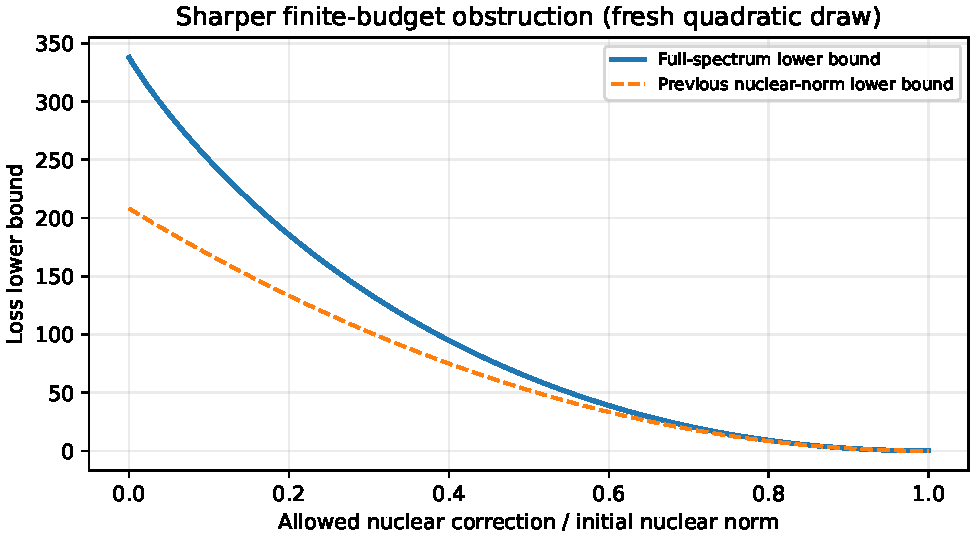
\includegraphics[width=.82\textwidth]{results/fanions/stronger_barrier.pdf}
\caption{Retaining the spectrum strengthens the earlier scalar nuclear
bound. This figure only displays the nuclear constraint; operator and
rank constraints can strengthen it further. Fresh draw, not saved training.}
\end{figure}

\section{Solvable rank dynamics and hybrid crossover scales}\label{sec:flow}

\subsection{An exact finite-step Fanion example}

Take $f(X)=\F{X}^2/2$, $X_0=sI_r$, and constant $\gamma=s/h$ with
$h$ a positive integer. Select the top $k$ positive residual singular
directions each step, stopping at zero. Let
$n_T=\min(kT,rh)=qr+p$, $0\leq p<r$. Then
\begin{equation}\label{eq:flatdiscrete}
 f(X_T)=\tfrac12\bigl[(r-p)(s-q\gamma)^2
                 +p(s-(q+1)\gamma)^2\bigr].
\end{equation}
Indeed the $k$ largest residuals are the least-served coordinates, so their
service counts differ by at most one. Before extinction,
\begin{equation}\label{eq:flatapprox}
 f(X_T)=\frac r2\left(s-\frac{k\gamma T}{r}\right)^2
               +\frac{\gamma^2p}{2}\left(1-\frac pr\right).
\end{equation}
The rounding remainder is at most $r\gamma^2/8$. This is an actual discrete
Fanion trajectory and proves an approximately exact dependence on $kT$,
with extinction after $\lceil rh/k\rceil$ steps. Momentum and variable
curvature are not part of this example.

\subsection{A whole-spectrum continuous model}

For the isotropic quadratic, consider the convexified spectral flow
$\dot X\in-\partial S_k(X)$. At a tie, this allows averages of tied
rank-$k$ maximizers. If $X_0=U\operatorname{diag}(s)V^\top$, its solution is
\begin{equation}\label{eq:flow}
 X(u)=U\operatorname{diag}(s_i-a_i(u))V^\top,\qquad
 a_i(u)=\min\{u,(s_i-\tau(u))_+\},
\end{equation}
where $\sum_i a_i(u)=\min\{ku,\sum_i\min(u,s_i)\}$.
Its exact extinction time is
\begin{equation}\label{eq:extinction}
 u_*^{\mathrm{P}}=\max\left\{s_1,\frac{\sum_i s_i}{k}\right\}.
\end{equation}

\begin{proof}
The formula is continuous and piecewise affine. On an interval with a
positive threshold, let $c$ corrections be capped at $u$ and let $j$ be
strictly between zero and $u$. Differentiating their sum $ku$ gives rate
one on the capped modes and rate $(k-c)/j$ on the tied residual plateau.
If $j=0$, then $c=k$ and only the capped modes move, at rate one.
This rate lies in $[0,1]$; the selected modes are the largest residuals, and
the total rate is $k$. Thus the negative derivative is in
$\partial S_k(X)$. When the nuclear constraint is inactive, every remaining
positive residual decreases at rate one; their number is at most $k$.
The expression is zero exactly when both $u\geq s_1$ and
$ku\geq\sum_i s_i$. Uniqueness follows from monotonicity of the
subdifferential of the convex function $S_k$.
\end{proof}

The crossover is $k\approx\nuc{X_0}/\op{X_0}$: below it the nuclear
budget gives $1/k$ improvement; above it the largest mode limits progress.
This is more informative than a uniform $r/k$ slogan. The continuous model
permits full-rank averages at ties, so \eqref{eq:flow} is not an exact
finite-step formula for a literal rank-$k$ implementation. It is a
convexified small-step model. Equation~\eqref{eq:flatdiscrete} supplies a
finite-step check in an important special case.

\subsection{F-Fanion flow is a time change of the plain flow}

For $a>0$, let $Z(u)$ be the plain flow just constructed and define, while
$Z(u)\ne0$,
\begin{equation}\label{eq:Ftimechange}
 c(u)=\exp\left\{-\frac ba\int_0^u\frac{dv}{\F{Z(v)}}\right\},\qquad
 t(u)=\frac1a\int_0^u c(v)\,dv,\qquad X(t(u))=c(u)Z(u).
\end{equation}
Differentiation gives
$\dot X\in-a\partial S_k(X)-bX/\F{X}$, exactly the convexified F-Fanion
flow. Its extinction time is $\lim_{u\uparrow u_*^{\mathrm{P}}}t(u)$, and is at
most both $u_*^{\mathrm{P}}/a$ and $\F{X_0}/b$ when $b>0$.
The first bound uses $c\leq1$; the second follows from
$-d\F{X}/dt=aS_k(X)/\F{X}+b\geq b$.
This statement is restricted to the isotropic quadratic and ideal continuous
oracles; it is not a theorem about general Kronecker Hessians.

\subsection{Flat-spectrum hybrids: exact crossover examples}

If $X_0=sQ$, with $Q$ square orthogonal, the averaged tied maximizer
$(k/r)Q$ makes the F-flow stay on the ray through $Q$. Hence
\begin{equation}\label{eq:hybridtimes}
 u_*^{\mathrm{P}}=\frac{rs}{k},\qquad
 t_*^{\mathrm{F}}=\frac{rs}{ak+b\sqrt r}.
\end{equation}
The low-rank F-family saturates at a time of order $\sqrt r$ instead of
$r/k$, and changing $k$ has little effect when $k\ll(b/a)\sqrt r$.
This attains the nuclear-capacity lower bound for that flow.

For S-Fanions the coordinate basis matters. If $Q$ is a normalized
Hadamard matrix, so every entry is $\pm1/\sqrt r$, then
$\sgn(Q)=\sqrt rQ$, and the S-flow on the same ray has
\begin{equation}\label{eq:Stime}
 t_*^{\mathrm{S}}=\frac{rs}{ak+b\eta r^{3/2}}.
\end{equation}
Such examples can be constructed at every power-of-two $r$ using the
Sylvester recursion. If instead $Q=I$, the denominator is
$ak+b\eta r$. The gradient singular spectrum is identical in these two
examples, but the sign term behaves differently. Entry density is therefore
necessary in an explanation of the S-family. These formulas use tied
averaged oracles and continuous time, as stated above.

For $r=500$, $a=b$, and the paper's $\eta=.01$, the dense-support crossover
scales are approximately 22.4 for F-Fanions and 111.8 for dense S-Fanions
with maximal entry uniformity. Gaussian-like entries insert a factor
$\sqrt{2/\pi}$, giving about 89.2 for the latter. These are model scales,
not fitted optimum ranks or predictions of exact threshold times.

\section{Comparison with the saved quadratic Fanions}\label{sec:data}

The file \path{code/long_run} contains all 17 methods, 500 saved losses each,
at iterations $0,10,\ldots,4990$. All these losses are finite. The initial
loss 302.896057 is common to every method. Muon, F-Muon, and S-Muon first
reach the saved $10^{-3}$ threshold at 1060, 910, and 890, respectively,
matching the manuscript's reported values.
The complete data and current-source settings are exported to
\path{results/fanions/saved_quadratic_summary.csv}; input hashes are retained
in \path{results/fanions/summary.json}.

\begin{figure}[ht]
\centering
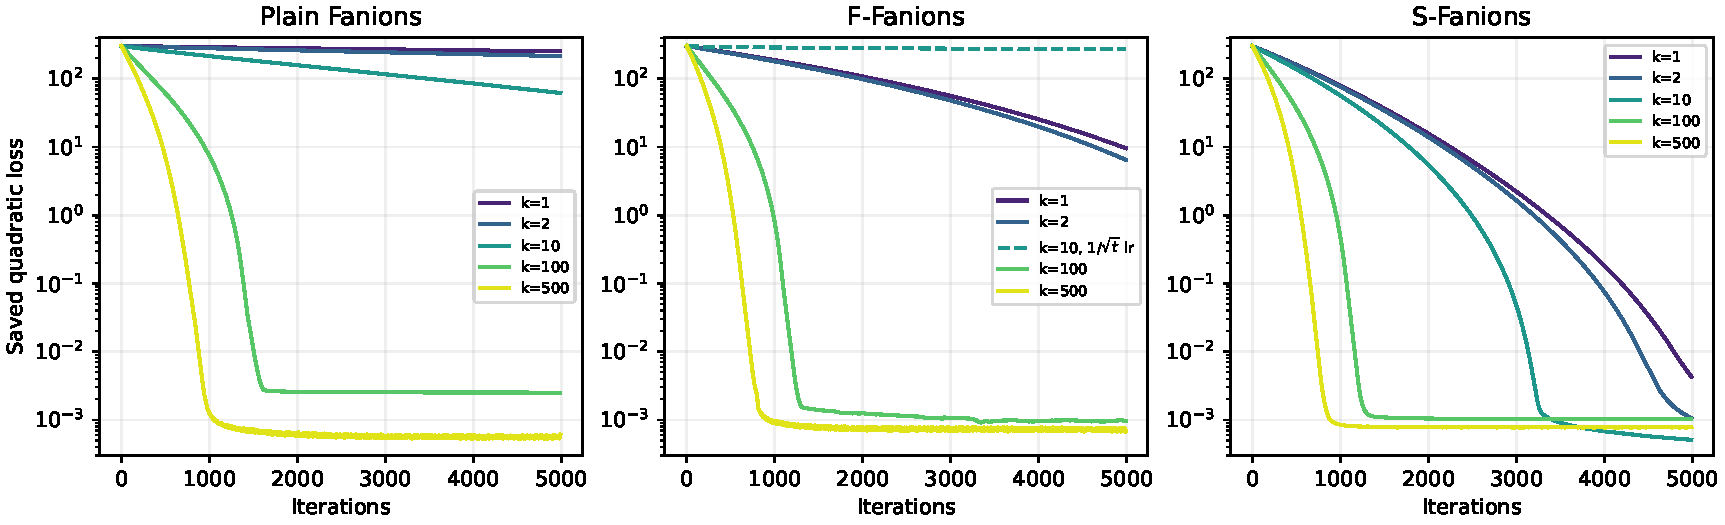
\includegraphics[width=\textwidth]{results/fanions/saved_fanion_families.pdf}
\caption{All five ranks in each saved family. The dashed F-Fanion-10 curve
has a different schedule in the current source. S-Fanion-10 reaches a
slightly lower saved loss floor than S-Muon; a universal ranking, at every
late-time threshold, is not the experimental pattern.}
\end{figure}

\subsection{The $kT$ prediction is unusually accurate at low ranks}

Compare the saved loss $f_k(t)$ with linearly interpolated Neon loss
$f_1(kt)$ over their common recorded horizon, excluding $t=0$.
No horizontal scaling parameter was fitted. The maximum absolute mismatch,
divided by the common initial loss, is:
\begin{center}
\begin{tabular}{rrrr}
\toprule
Rank & Compared points & Last $t$ & Maximum mismatch\\
\midrule
2 & 249 & 2490 & $0.000252\%$\\
10 & 49 & 490 & $0.01884\%$\\
100 & 4 & 40 & $1.8583\%$\\
\bottomrule
\end{tabular}
\end{center}
The rank-2 overlap is particularly striking. The rank-100 comparison has
only four noninitial points and does not justify extrapolating its accuracy.
These are same-problem saved traces, not comparisons to the fresh draw used
for the lower-bound table. They support a low-rank budget-limited regime;
they do not prove that the isotropic-flow equation governs the actual
anisotropic, momentum-driven quadratic.

\begin{figure}[ht]
\centering
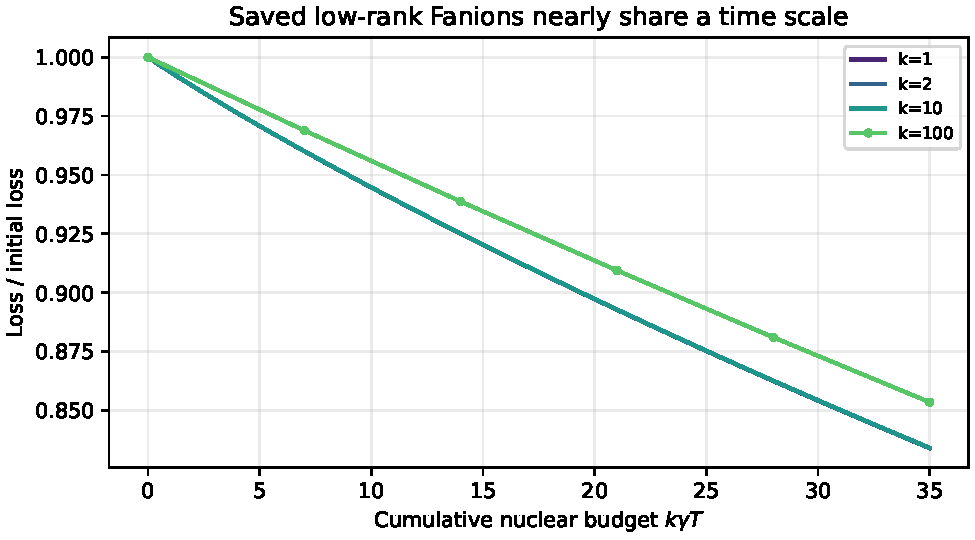
\includegraphics[width=.82\textwidth]{results/fanions/rank_time_collapse.pdf}
\caption{The plain family, plotted against $k\gamma T$ over the shared
Neon horizon. Rank-100 points show the beginning of a departure.}
\end{figure}

\subsection{First-order projections also distinguish the hybrids}

The initial saved gradient has
$\op{G_0}=2.019055$, $\F{G_0}=16.030416$, and
$\nuc{G_0}=250.871033$.
Ignoring curvature and gradient change over the first ten updates gives
$10\gamma\phi_1(G_0)$. For the sign term only, approximate
$\ent{G_0}$ by $\sqrt{2/\pi}\sqrt d\F{G_0}$, the expectation for isotropic
Gaussian entries at the same variance scale. This is a distributional model,
not an observed entrywise norm. The comparisons are:
\begin{center}
\begin{tabular}{lrrr}
\toprule
Method & Saved ten-step loss drop & Projection model & Relative error\\
\midrule
Neon & 0.140320 & 0.141334 & $0.723\%$\\
F-Neon & 1.350525 & 1.353710 & $0.236\%$\\
S-Neon & 3.606323 & 3.628414 & $0.613\%$\\
\bottomrule
\end{tabular}
\end{center}
At the first step, positive scalar momentum scaling does not change any of
the ideal directions. The small ten-step discrepancies are consistent with
the short-interval projection model. This local agreement does not validate
the Gaussian approximation or constant projected dynamics throughout training.

\section{When should the next rank help?}\label{sec:marginal}

At a common point with an exact gradient, let a valid directional quadratic
upper model have curvature $C_k>0$ along $D_k(G)$. Its best scalar-step
decrease certificate is $S_k(G)^2/(2C_k)$. Therefore
\begin{equation}\label{eq:marginal}
 \frac{S_{k+1}^2}{C_{k+1}}\geq\frac{S_k^2}{C_k}
 \quad\Longleftrightarrow\quad
 \frac{C_{k+1}}{C_k}\leq
       \left(1+\frac{\sigma_{k+1}}{S_k}\right)^2.
\end{equation}
With Frobenius curvature $C_k=Lk$, put
$q_k=S_k^2/(k\F{G}^2)$. Then the next rank helps this certificate precisely
when
\begin{equation}\label{eq:qthreshold}
 \frac{\sigma_{k+1}}{S_k}\geq\sqrt{1+1/k}-1
 =\frac{1}{k(\sqrt{1+1/k}+1)}.
\end{equation}
For $\sigma_i$ proportional to $i^{-p}$ and $0\leq p<1$,
$S_k$ is asymptotic to a constant times $k^{1-p}$, so the large-$k$ rank
profile is proportional to $k^{1-2p}$ in the range $1\ll k\ll r$, apart
from a normalizing factor independent of $k$. Spectra flatter than the
$p=1/2$ boundary favor more ranks in this
model; faster decay eventually penalizes additional weak modes. This is a
statement about the certificate's spectral term, not a universal optimizer
ordering.

\subsection{Nonmonotone hybrid rank curves even for a flat spectrum}

Suppose every singular value of $G$ equals $s>0$ and $a>0$.
For exact rank-$k$ directions, put $t=b/a$. The F-Fanion cosine squared is
\begin{equation}\label{eq:flatFprofile}
 q_k^{\mathrm F}=
 \frac{(k/\sqrt r+t)^2}{k+t^2+2tk/\sqrt r}.
\end{equation}
As a function of real $k>0$ this decreases until
$k_{\min}=tr/(\sqrt r+2t)$ and increases thereafter; when
$k_{\min}<1$ the admissible ranks are on its increasing part.
For $r=64$, $a=b$, its values at $k=1,5,64$ are respectively
$0.5625$, $0.364224$, and $1$. Thus a low-rank F-hybrid can beat an
intermediate rank even though the full-rank hybrid has the best score.
The minimum for equal coefficients is near $\sqrt r$, the same scale as
the dense-support crossover found earlier.

For S-Fanions at a flat Hadamard gradient, the same expression holds with
$t=(b/a)\eta r$; at a flat diagonal gradient, use
$t=(b/a)\eta\sqrt r$. These are exact common-gradient scores and do not
require averaged tie choices. They illustrate how the interior rank curve
changes with the hybrid and the coordinate basis. The scalar step is
optimized separately in these scores; an actual fixed learning rate must
instead be assessed with the next calculation.

\begin{figure}[ht]
\centering
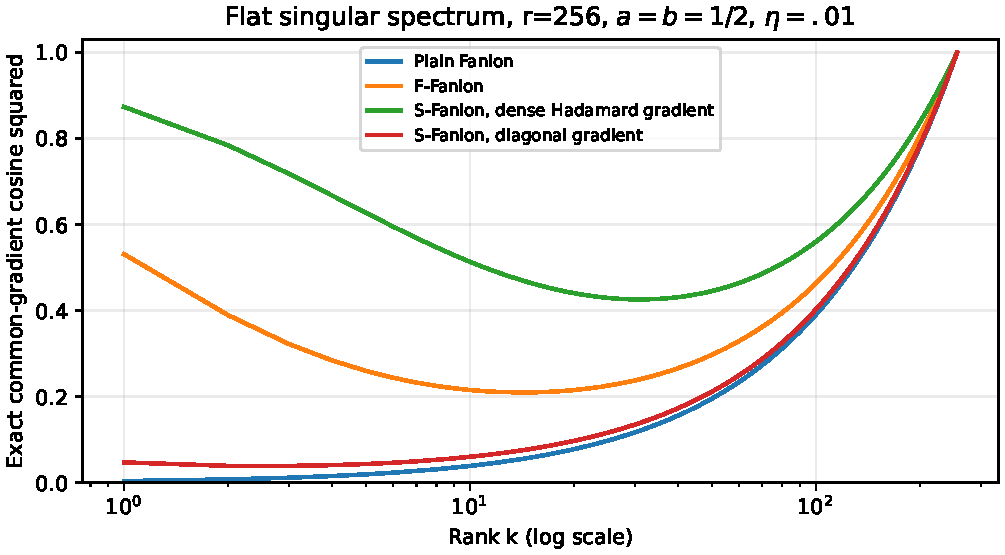
\includegraphics[width=.86\textwidth]{results/fanions/flat_hybrid_rank_profiles.pdf}
\caption{Exact rank profiles at flat-spectrum gradients. The plain and F
profiles are invariant under orthogonal changes of basis. The two S
profiles have the same singular spectrum and different entry structures.
All full-rank directions here are parallel to the gradient.}
\end{figure}

\paragraph{A fixed learning rate asks a different question.}
For a quadratic with Hessian operator $\mathcal H$, set
$P=u_{k+1}(H)v_{k+1}(H)^\top$. For any of the three families, let
$D_k'$ be its direction, and let $a'=1$ for the plain family and $a'=a$
for either hybrid. Increasing rank changes the direction by $a'P$ and its
actual one-step loss reduction by
\begin{equation}\label{eq:fixedmarginal}
 \gamma a'\ip{G}{P}
 -\frac{\gamma^2}{2}
  \left(2a'\ip{D_k'}{\mathcal H P}
              +(a')^2\ip{P}{\mathcal H P}\right).
\end{equation}
When $H=G$ and $\mathcal H=L I$, the plain criterion is simply
$\sigma_{k+1}>L\gamma/2$. For the F-family it is
\[
 \sigma_{k+1}\left(1-\frac{L\gamma b}{\F{G}}\right)
 >\frac{L\gamma a}{2},
\]
assuming $a>0$ and a positive parenthesis. For the S-family the cross term
also contains $\ip{\sgn(G)}{P}$. Momentum can make
$\ip{G}{P(H)}$ differ from $\sigma_{k+1}(G)$ or even become negative.
This equation identifies the exact measurements needed for every new rank.

For the manuscript's quadratic,
$\mathcal H D=MDN$ and
$C_k=\sum_{i,j\leq k}(u_i^\top M u_j)(v_i^\top N v_j)$.
The cross terms are real and need not all be positive. Assuming curvature is
just $k$ times the first-mode curvature is an additional modeling assumption.

\section{What the norm logs can and cannot say about Fanion-5}\label{sec:moments}

The CIFAR logs contain only $\op{G}$, $\F{G}$, and $\nuc{G}$, rather than
all singular values or the actual momentum input. They determine $S_1$ and
$S_r$ but not $S_5$. This is an identifiable mathematical limitation.

\subsection{Identical recorded norms, opposite rank-5 conclusions}

Take $r=64$, $\sigma_1=1$, $\sum_i\sigma_i=16$, and
$\sum_i\sigma_i^2=6.5$. There are two positive spectra with these moments:
one has four elevated singular values below the first, the other has twenty.
They can be constructed explicitly by choosing two levels in the remaining
63 entries to match their sum and squared sum. Their scores are:
\begin{center}
\begin{tabular}{lrrrr}
\toprule
Spectrum & $S_5$ & $q_5$ & $q_r$ & $q^{\mathrm{F}}_5$\\
\midrule
Four elevated modes & 4.640222 & 0.662513 & 0.615385 & 0.824956\\
Twenty elevated modes & 2.978569 & 0.272981 & 0.615385 & 0.563958\\
\bottomrule
\end{tabular}
\end{center}
For both, $q^{\mathrm{F}}_r=0.682593$ when $a=b=1/2$, using
\[
 q_k^{\mathrm{F}}=\frac{(aS_k/\F{G}+b)^2}
 {a^2k+b^2+2abS_k/\F{G}}.
\]
Thus both the plain and F-family rank-5 versus full-rank comparisons reverse
while all three recorded norms remain identical. These are exact
Frobenius-curvature comparisons at a common gradient; any stronger inference
about actual training would need more information.

\begin{figure}[ht]
\centering
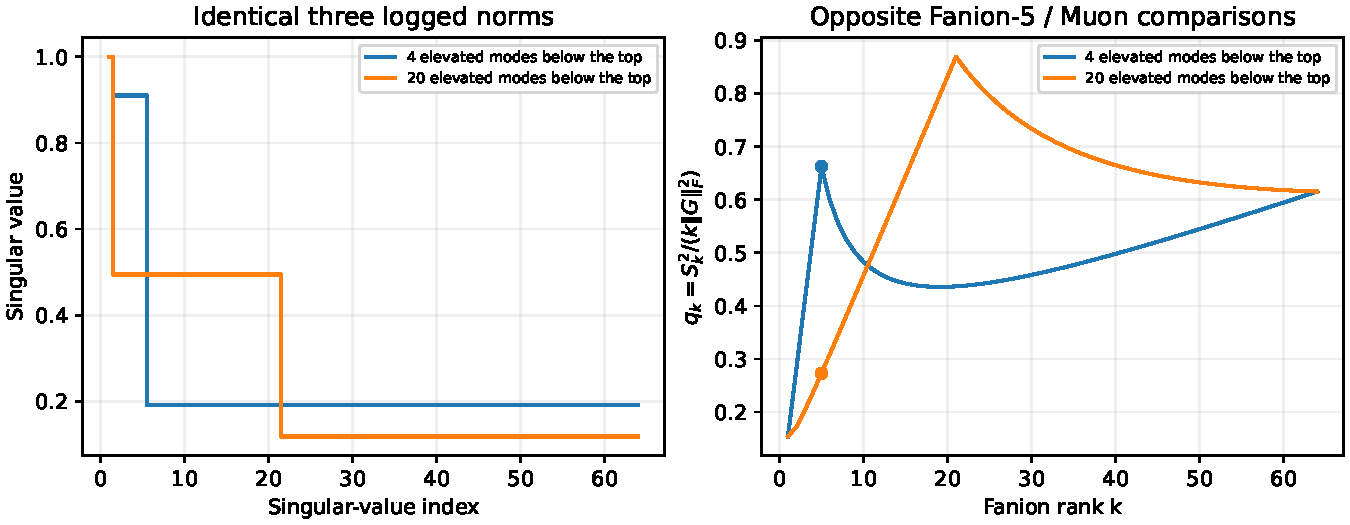
\includegraphics[width=\textwidth]{results/fanions/same_moments.pdf}
\caption{The same three gradient norms admit opposite intermediate-rank
comparisons. The score equals the cosine squared of the ideal update with
the gradient; the best isotropic quadratic decrease is
$q_k\F{G}^2/2$.}
\end{figure}

\subsection{Safe intervals from the existing three norms}

For $1<k<r$, write $a_0=\op{G}$, $S=\nuc{G}$, $Q=\F{G}^2$,
$n=r-1$, $p=k-1$, $q=r-k$, $A=S-a_0$, $V=Q-a_0^2$.
Then $a_0+L_k\leq S_k\leq a_0+U_k$, where
\[
 h_-=\frac{pa_0+A-\sqrt{(pa_0+A)^2-4pV}}{2}.
\]
\begin{equation}\label{eq:momentbounds}
\begin{aligned}
 L_k&=\max\{pA/n,\ A-qa_0,\ 0,\ h_-\},\\
 U_k&=\min\left\{pa_0,\ A,\
 \frac{pA}{n}+\sqrt{\frac{pq}{n}\left(V-\frac{A^2}{n}\right)}\right\}.
\end{aligned}
\end{equation}
These intervals are valid but need not be the tightest possible.
For their proof, put $H=\sum_{i=2}^k\sigma_i$. Sorting gives
$H\geq pA/n$ and $H\geq A-qa_0$. Cauchy--Schwarz on the two groups gives
$V\geq H^2/p+(A-H)^2/q$, yielding the upper bound. Conversely
the head squares sum to at most $a_0H$, and each tail singular value is at
most $H/p$, so
$V\leq a_0H+H(A-H)/p$. Its smaller quadratic root gives the remaining
lower bound.

For the predeclared reference file
\path{code/cifar_norms/grad_norms_Muon_run0_20251208_162732.csv},
the six convolution layers contribute 1,500 gradient snapshots.
Their ranks, inferred from the current network definition in
\path{code/cifar_bench/norm_logger_airbench.py}, are 64 for the first two
layers and 256 for the remaining four; this architecture assumption and its
source hash are retained with the results.
Using \eqref{eq:momentbounds}, Muon's common-point Frobenius certificate
exceeds the \emph{largest allowed} Fanion-5 certificate in 21.2\% of them.
The reverse is certified in 0.47\%; most comparisons remain unresolved.
For the F-family, F-Muon over F-Fanion-5 is certified in only 0.73\%.
These fractions refer to one trajectory's surrogate comparisons, not to
fractions of runs where one optimizer won. The individual intervals and
layerwise summaries are exported for all $k$ in
$\{1,2,5,10,\min(100,r),r\}$.

Only eight of the 250 loss rows in this reference file are finite; all norm
values used are finite. No loss-rate fit is made to these logs. They are
also different runs from the manuscript's eight-epoch CIFAR accuracy table.

\section{How to turn this into a stronger paper result}

\paragraph{A defensible result already available.}
Theorem~\ref{thm:all}, Proposition~\ref{prop:tracking}, and
Theorem~\ref{thm:waterfill} are proved bounds for every rank and hybrid
family. The exact flow and finite flat example explain when their rank
dependence is attainable. The saved low-rank time comparison and the
schedule audit are direct evidence specific to this repository.
The short fragment \path{paper_insert_fanions.tex} supplies a candidate
section without changing the submission.

\paragraph{The most useful next measurement.}
At common saved model states, record the actual momentum matrix $H$,
an independent gradient estimate $G$, and the actual implemented directions
for each rank. Save $S_k(H)$ and $\ip{G}{D_k(H)}$ for every desired $k$;
three aggregate norms cannot replace them. For S-hybrids also record
$\ent{H}$ and its sign cross terms. Estimate directional curvature and
pairwise cross terms using Hessian-vector products or controlled loss probes
at several step lengths. Evaluate both the frozen-state score
$\pos{\ip{G}{D}}^2/C(D)$ and the actual scheduled decrease
$\gamma\ip{G}{D}-\gamma^2C(D)/2$.

This would test a pre-specified rank curve, including the marginal condition
\eqref{eq:fixedmarginal}, instead of assuming that its endpoints determine
the interior. Validation accuracy still needs a generalization argument;
an optimization convergence bound alone does not imply an accuracy ordering.

\paragraph{Relation to existing literature.}
The support-function/descent and best singular-approximation ingredients are
standard. \href{https://arxiv.org/html/2510.09827}{Crawshaw et al.} develop a norm-based view that
also makes layerwise aggregation and update normalization explicit.
\href{https://arxiv.org/html/2606.15702v1}{Ma, Zhang, and He} analyze Schatten ball and regularization
oracles with momentum, minibatching, and multiple blocks. Their reported
stationarity uses the corresponding dual Schatten norm; comparing methods
on a common Frobenius target requires retaining norm conversions and
structural constants. Our sets $C_k$ and their hybrid Minkowski sums make
the manuscript's discrete rank parameter explicit. We make no priority
claim for the general analysis or a claim that the cited work establishes
a universal Fanion ordering. The first note discusses the other related
Muon and structured-optimization papers.

\paragraph{Reproduction and numerical checks.}
Run \path{python theory_attempts/fanion_analysis.py}, then
\path{python theory_attempts/build_report.py --stem fanion_followup}.
The analysis uses NumPy and Matplotlib on CPU. It checks 160 moment
intervals, 160 comparisons to the earlier scalar barriers, 480 actual
quadratic trajectory barriers, 2,482 flat finite-step identities, 160
continuous-flow support identities, 480 all-family oracle inequalities,
and 400 Nesterov unrolling/tracking identities. These numerical checks
support the implementation; the mathematical guarantees rest on the proofs
and assumptions above. The output JSON includes source hashes and complete
numbers. No new neural-network training, checkpoint recovery, or original
experiment replication is claimed.

\section*{References}
\begin{enumerate}
\item
M. Crawshaw, C. Modi, M. Liu, and R. M. Gower.
\emph{An Exploration of Non-Euclidean Gradient Descent: Muon and its Many
Variants}. arXiv:2510.09827, 2025.
\url{https://arxiv.org/html/2510.09827}.
\item
B. Ma, J. Zhang, and C. He.
\emph{Schattor: Schatten-family methods for deep learning optimization}.
arXiv:2606.15702, 2026.
\url{https://arxiv.org/html/2606.15702v1}.
\end{enumerate}
\end{document}
